\setcounter{chapter}{15}
\chapter{Inference for Simple Linear Regression}

\section{Inference on Regression}

In previous chapters, we focused on estimating regression parameters and interpreting the fitted line. In this chapter, we take a step further by conducting formal inference on the slope and intercept of a simple linear regression model. We examine the distribution of errors, assess variability, and introduce the idea of using hypothesis tests and confidence intervals to evaluate whether the linear relationship observed in the data is statistically significant.

\vspace{1em}
We begin by introducing the regression model and exploring the assumptions necessary to perform inference on the coefficients, particularly the slope.

\[
Y = \beta_0 + \beta_1 X + \varepsilon, \quad \varepsilon \sim \mathcal{N}(0, \sigma^2)
\]

Can perform inference on $\beta_0$ and $\beta_1$, however we are usually more interested in $\beta_1$. \\

What does the error term $\varepsilon \sim \mathcal{N}(0, \sigma^2)$ mean? \\
\textbf{At each} value of $X$, the errors are distributed normally with a mean of zero and a constant variance.

\begin{figure}[H]
  \centering
  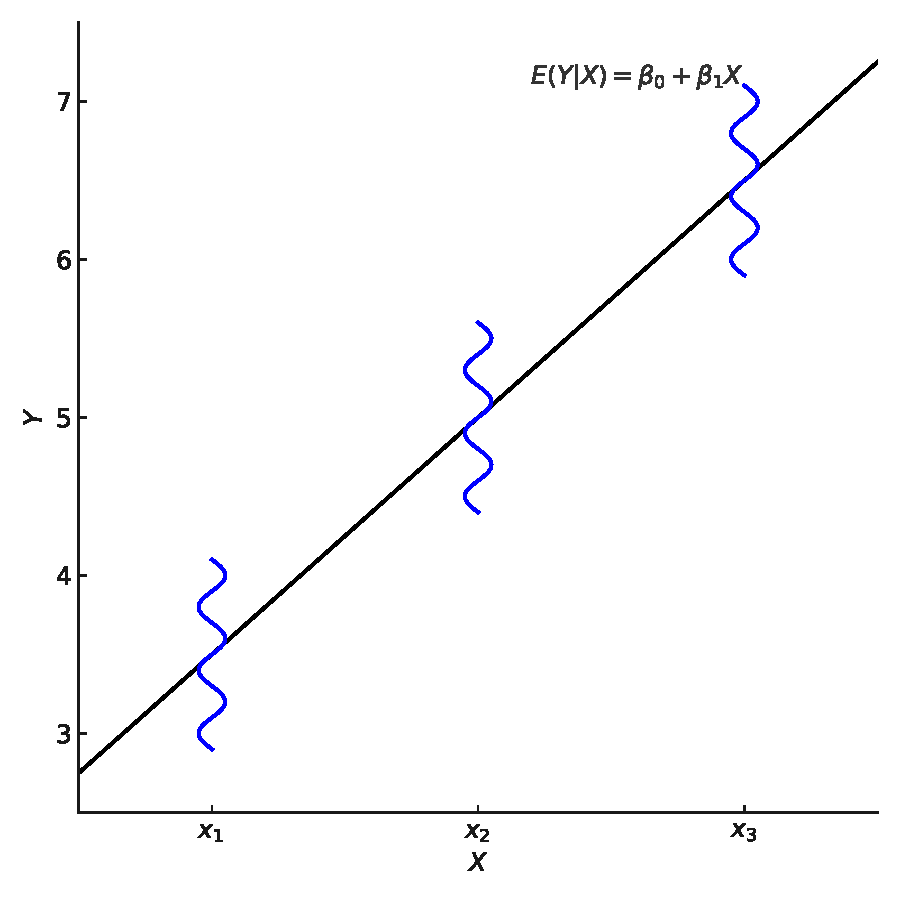
\includegraphics[width=0.6\textwidth]{section16/images/regression_model.pdf}
  \caption{Regression line with normal errors at each $X$}
\end{figure}

Can verify with residual plots (assumptions).

We estimate $\sigma^2$ with a value we call $S^2$ and use $S^2$ for inference.

\subsection*{Estimating Variance in Linear Regression}

\[
Y = \beta_0 + \beta_1 X + \varepsilon, \quad \varepsilon \sim \mathcal{N}(0, \sigma^2)
\]

\textbf{Estimate $\sigma^2$ with $S^2$}:

\[
S^2 = \frac{\sum_{i=1}^n e_i^2}{n - 2}
= \frac{\sum_{i=1}^n (y_i - \hat{y}_i)^2}{n - 2}
= \frac{SSE}{n - 2}
\]

\hfill \textcolor{red}{\textit{notice similarity}}

\[
S_x^2 = \frac{\sum_{i=1}^n (x_i - \bar{x})^2}{n - 1}
\quad \textcolor{blue}{\text{(sample variance, }\bar{x} \text{ estimated)}}
\]

\[
S = +\sqrt{S^2}
\quad \textcolor{blue}{\text{(estimate of standard deviation)}} \\
\]

\vspace{1em}

\textbf{In calculating $S^2$, why do we divide by $n-2$?}

Since we estimate 2 unknown parameters in the model (both $\beta_0$ and $\beta_1$), which are used in the calculation of $S^2$.

\begin{tcolorbox}[colback=yellow!5, colframe=yellow!50!black,
title={Equation of the Least-Squares Regression Line}, 
boxrule=0.5pt, sharp corners, breakable]

We have data on an explanatory variable $x$ and a response variable $y$ for $n$ individuals. From the data, calculate the means $\bar{x}$ and $\bar{y}$ and the standard deviations $S_x$ and $S_y$ of the two variables, and their correlation $r$. The least-squares regression line is the line:

\[
\hat{y} = b_0 + b_1 x
\]

with \textit{slope}

\[
b_1 = r \frac{S_y}{S_x}
\]

and \textit{intercept}

\[
b_0 = \bar{y} - b_1 \bar{x}
\]

\end{tcolorbox}

\begin{definition}[Least-Squares Regression Line]
The \textbf{least-squares regression line} of $y$ on $x$ is the line that makes the sum of the squares of the vertical distances of the data points from the line as small as possible.
\end{definition}

\begin{example}
Suppose an appliance store conducts a 5-month experiment to determine the effect of advertising on sales revenue. The results are shown in a table below. The relationship between sales revenue, $y$, and advertising expenditure, $x$, is hypothesized to follow a first-order linear model, that is,

\[
y = \beta_0 + \beta_1 x + \varepsilon
\]

where

\begin{align*}
y & = \text{dependent variable} \\
x & = \text{independent variable} \\
\beta_0 & = \text{$y$-intercept} \\
\beta_1 & = \text{slope of the line} \\
\varepsilon & = \text{error variable}
\end{align*}


\begin{table}[H]
\centering
\small
\renewcommand{\arraystretch}{1.2}
\setlength{\tabcolsep}{4pt} % tighter columns
\begin{tabular}{p{1.5cm} p{3cm} p{3cm}}
\toprule
\textbf{Month} &
\shortstack{\textbf{Advertising} \\ \textbf{Expenditure} \\ $x$ (\$ hundreds)} &
\shortstack{\textbf{Sales} \\ \textbf{Revenue} \\ $y$ (\$ thousands)} \\
\midrule
1 & 1 & 1 \\
2 & 2 & 1 \\
3 & 3 & 2 \\
4 & 4 & 2 \\
5 & 5 & 4 \\
\bottomrule
\end{tabular}
\end{table}



The question is this: How can we best use the information in the sample of five observations in our table to estimate the unknown $y$-intercept $\beta_0$ and slope $\beta_1$?

\vspace{1em}

We are given:
\[
\bar{x} = 3, \quad \bar{y} = 2, \quad S_x = 1.5811, \quad S_y = 1.2247, \quad S_{xy} = 1.75
\]

Then, the slope of the least squares line is

\[
b_1 = r \frac{S_y}{S_x} = (0.9037) \left( \frac{1.2247}{1.5811} \right) = 0.7
\]

and

\[
b_0 = \bar{y} - b_1 \bar{x} = 2 - (0.7)(3) = -0.1
\]

The least squares line is thus:

\[
\hat{y} = -0.1 + 0.7x
\]
\end{example}

\subsection*{The Regression Model}

We have $n$ observations on an explanatory variable $x$ and a response variable $y$. Our goal is to study or predict the behavior of $y$ for given values of $x$.

\begin{itemize}
  \item For any fixed value of $x$, the response $y$ varies according to a Normal distribution. Repeated measures $y$ are independent of each other.
  
  \item The mean response $\mu_y$ has a straight-line relationship with $x$:  
  $\mu_y = \beta_0 + \beta_1 x$.  
  The slope $\beta_1$ and intercept $\beta_0$ are \textbf{unknown} parameters.
  
  \item The standard deviation of $y$ (call it $\sigma$) is the same for all values of $x$.  
  The value of $\sigma$ is \textbf{unknown}.  
  The regression model has three parameters, $\beta_0$, $\beta_1$, and $\sigma$.
\end{itemize}

Thus, if
\[
\hat{y}_i = \hat{\beta}_0 + \hat{\beta}_1 x_i
\]
is the predicted value of the $i$th $y$ value, then the deviation of the observed value $y_i$ from $\hat{y}_i$ is the difference $y_i - \hat{y}_i$ and the sum of squares of deviations to be minimized is

\[
SSE = \sum_{i=1}^{n} (y_i - \hat{y}_i)^2 = \sum_{i=1}^{n} [y_i - (\hat{\beta}_0 + \hat{\beta}_1 x_i)]^2.
\]

The quantity \textit{SSE} is also called the \textbf{sum of squares for error}.
\begin{align*}
\text{Fitted Value:} \quad & \hat{y}_i = \hat{\beta}_0 + \hat{\beta}_1 x_i \\
\text{Residual:} \quad & \hat{\varepsilon}_i = y_i - \hat{y}_i
\end{align*}

The \textbf{regression standard error} is

\[
s = \sqrt{\frac{1}{n - 2} \sum \text{residual}^2} 
= \sqrt{\frac{1}{n - 2} \sum_{i=1}^{n} (y_i - \hat{y}_i)^2} 
= \sqrt{\frac{SSE}{n - 2}}
\]

Use $s$ to estimate the \textbf{unknown} $\sigma$ in the regression model.\\

The standard error of $\hat{\beta}_1$ is the standard deviation of the sampling distribution of $\hat{\beta}_1$ (estimate of slope $\beta_1$):

\[
SE(\hat{\beta}_1) = \frac{s}{\sqrt{\sum_{i=1}^{n} (x_i - \bar{x})^2}} 
= \frac{s}{\sqrt{(n - 1) s_x^2}}
\]

\vspace{1em}

\textbf{Confidence Interval for the Slope}

\[
\hat{\beta}_1 \pm t_{(n-2, \, \alpha/2)} \cdot SE(\hat{\beta}_1)
\quad = \quad 
\hat{\beta}_1 \pm t_{(n-2, \, \alpha/2)} \cdot \frac{s}{\sqrt{\sum_{i=1}^{n} (x_i - \bar{x})^2}}
\]

\begin{example}[continued]
Revisit the example on advertising and sales and construct a 95\% confidence interval on the slope. Provide an interpretation of the CI.

From earlier:
\[
\hat{y} = -0.1 + 0.7x
\]

\begin{center}
\begin{tabular}{cccccc}
\toprule
\textbf{$x$} & \textbf{$y$} & \textbf{$\hat{y}$} & \textbf{$y - \hat{y}$} & \textbf{$(y - \hat{y})^2$} & \textbf{$(x - \bar{x})^2$} \\
\midrule
1 & 1 & 0.6 & 0.4 & 0.16 & 4 \\
2 & 1 & 1.3 & -0.3 & 0.09 & 1 \\
3 & 2 & 2.0 & 0.0 & 0.00 & 0 \\
4 & 2 & 2.7 & -0.7 & 0.49 & 1 \\
5 & 4 & 3.4 & 0.6 & 0.36 & 4 \\
\bottomrule
\end{tabular}
\end{center}

\vspace{1em}
We are given:
\[
\sum x_i = 15, \quad \bar{x} = \frac{15}{5} = 3, \quad SSE = 1.10, \quad \sum (x_i - \bar{x})^2 = 10
\]

\vspace{1em}
\textbf{Step 1: Estimate variance and standard deviation}
\[
s^2 = \frac{SSE}{n-2} = \frac{1.10}{5 - 2} = 0.3667
\quad \Rightarrow \quad
s = \sqrt{0.3667} = 0.6055
\]

\vspace{1em}
\textbf{Step 2: Compute standard error of $\hat{\beta}_1$}
\[
SE(\hat{\beta}_1) = \frac{s}{\sqrt{\sum (x_i - \bar{x})^2}} 
= \frac{0.6055}{\sqrt{10}} = 0.1914
\]

\vspace{1em}
\textbf{Step 3: Determine critical $t$-value}

\[
n - 2 = 3, \quad \alpha = 0.05, \quad \alpha/2 = 0.025
\Rightarrow \quad
t_{(3, 0.025)} = 3.182
\]

\vspace{1em}
\textbf{Step 4: Construct CI for the slope}
\[
\hat{\beta}_1 \pm t_{(n-2, \alpha/2)} \cdot SE(\hat{\beta}_1)
= 0.7 \pm 3.182 \cdot 0.1914 = 0.7 \pm 0.6092
\]

\[
\Rightarrow \text{CI: } (0.0908, \; 1.3092)
\]

\vspace{1em}
\textbf{Interpretation:}  
We are 95\% confident the slope ($\beta_1$) for this model lies between 0.0908 and 1.3092.
\end{example}
\subsection*{Interpreting Confidence Intervals for $\beta_1$}

\begin{center}
\begin{tabular}{rl}
\textbf{Suppose CI:} & $(-, -)$ \\
& Suggests $\beta_1$ has a \textbf{negative} sign. \\
& Suggests negative correlation, potentially good model. \\
\\
\textbf{Suppose CI:} & $(+, +)$ \\
& Suggests $\beta_1$ has a \textbf{positive} sign. \\
& Suggests positive correlation, potentially good model. \\
\\
\textbf{Suppose CI:} & $(-, +)$ \\
& $\beta_1 = 0$ is plausible. \\
& Suggests \textbf{no linear relationship} between $x$ and $y$.
\end{tabular}
\end{center}

\vspace{0.5em}
In cases where the CI does not contain zero, we can infer the sign of the slope (just not the steepness).\\

The \textbf{regression standard error} is

\[
s = \sqrt{\frac{1}{n - 2} \sum_{i=1}^n (y_i - \hat{y}_i)^2} = \sqrt{\frac{SSE}{n - 2}} = \sqrt{\frac{1.1}{3}} = 0.6055
\]

Use $s$ to estimate the \textbf{unknown} $\sigma$ in the regression model.\\

A level $C$ confidence interval for the slope $\beta_1$ of the true regression line is

\[
b_1 \pm t^* SE_{b_1}
\]

In this formula, the standard error of the least-squares slope $b$ is

\[
SE_{b_1} = \frac{s}{\sqrt{\sum (x_i - \bar{x})^2}} = \frac{s}{\sqrt{(n - 1) S_x^2}}
\]

and $t^*$ is the critical value for the $t(n - 2)$ density curve with area $C$ between $-t^*$ and $t^*$.

\begin{tcolorbox}[
  colback=yellow!5,
  colframe=yellow!50!black,
  title={Hypothesis Test on the Slope $\beta_1$},
  boxrule=0.4pt, sharp corners, breakable
]

\textbf{Hypotheses:}
\begin{align*}
H_0\!: \beta_1 = 0 \quad & \text{vs.} \quad H_a\!: \beta_1 > 0 \\
H_0\!: \beta_1 = 0 \quad & \text{vs.} \quad H_a\!: \beta_1 < 0 \\
H_0\!: \beta_1 = 0 \quad & \text{vs.} \quad H_a\!: \beta_1 \neq 0 \quad \text{\textit{(most common)}}
\end{align*}

\vspace{0.75em}
\textbf{Test Statistic:}
\[
t = \frac{\hat{\beta}_1 - 0}{SE(\hat{\beta}_1)} = \frac{\hat{\beta}_1}{\dfrac{s}{\sqrt{\sum_{i=1}^n (x_i - \bar{x})^2}}}
\]

\vspace{0.75em}
\textbf{Reference distribution:} $t$ distribution with $n - 2$ degrees of freedom.

\vspace{1em}
\textit{Note:} A test statistic always follows the form:
\[
\text{test stat} = \frac{\text{statistic} - \text{hypothesized value}}{\text{SE(statistic)}}
\]

\end{tcolorbox}

\begin{example}[continued]
For the advertising example, perform a two-sided hypothesis test on the slope.

\textbf{Hypotheses:}
\[
H_0\!: \beta_1 = 0 
\qquad 
H_a\!: \beta_1 \neq 0
\]

\vspace{0.5em}
\textbf{Test Statistic:}
\[
t^* = \frac{\hat{\beta}_1 - 0}{\dfrac{s}{\sqrt{\sum (x_i - \bar{x})^2}}}
= \frac{0.7 - 0}{0.6055 / \sqrt{10}} = 3.6558
\]

\vspace{0.5em}
\textbf{Reference Distribution:} 
$t$ distribution with $n - 2 = 5 - 2 = 3$ degrees of freedom.

\vspace{0.5em}
\textbf{Decision Rule:} 

Using a two-tailed test:
\[
\text{p-value} = 2 \cdot P(T_3 > 3.6558) < 0.01 \Rightarrow \text{p-value} < 0.05
\]

\textbf{Conclusion:}  
Since $p$-value $< 0.05$, we reject $H_0$ and conclude $H_a\!: \beta_1 \neq 0$.

\textit{Interpretation:}  
The slope should be included in the model. There is significant evidence of a linear relationship between advertising and sales revenue.\\

For the advertising-sales example, a 95\% Confidence Interval for the slope $\beta_1$ is
\[
0.7 \pm 3.182 \left( \frac{0.6055}{\sqrt{10}} \right)
\]
\[
0.7 \pm 0.6092
\]

Thus, we estimate with 95\% confidence that the interval from 0.0908 and 1.3092 includes the parameter $\beta_1$.
\end{example}
We can also test hypotheses about the slope $\beta_1$. The most common hypothesis is

\[
H_0 : \beta_1 = 0.
\]

A regression line with slope 0 is horizontal. That is, the mean of $y$ does not change at all when $x$ changes. So this $H_0$ says that there is no true linear relationship between $x$ and $y$.
\begin{tcolorbox}[title=\textbf{Testing the Hypothesis for \boldmath$\beta_1$},
colback=yellow!10,
colframe=black!45,
coltitle=black,
fonttitle=\bfseries,
breakable]

To test the hypothesis $H_0 : \beta_1 = 0$, compute the $t$ statistic
\[
t = \frac{b_1}{SE_{b_1}}.
\]

In terms of a random variable $T$ having the $t(n - 2)$ distribution, the P-value for a test of $H_0$ against:
\begin{align*}
H_a : \beta_1 \ne 0 & \quad \text{is } 2P(T > |t|). \\
H_a : \beta_1 > 0 & \quad \text{is } P(T > t). \\
H_a : \beta_1 < 0 & \quad \text{is } P(T < t).
\end{align*}

\end{tcolorbox}

\begin{example}[continued]
\[
\alpha = 0.05
\]
\begin{enumerate}
    \item[1)]  $H_0: \beta_1 = 0 \quad \text{vs} \quad H_a: \beta_1 > 0$
    \item[2)] $t^* = \frac{b_1}{SE_{b_1}} = \frac{0.7}{0.1914} = 3.6572$
    \item[3)] $P\text{-value} = P(T > t) = P(T > 3.6572) \quad \text{d.f.} = n - 2 = 5 - 2 = 3.$\\
    Using t-distribution table, $0.01 < P\text{ value} < 0.025$
    \item[4)] Since $P\text{-value} < \alpha = 0.05$, we reject $H_0$.
\end{enumerate}

Our example (different $H_a$)
\[
\alpha = 0.05
\]
\begin{enumerate}
    \item[1)] $H_0: \beta_1 = 0 \quad \text{vs} \quad H_a: \beta_1 \neq 0$
    \item[2)] $t^* = \frac{b_1}{SE_{b_1}} = \frac{0.7}{0.1914} = 3.6572$
    \item[3)] $P\text{-value} = 2P(T > |t|) = 2P(T > 3.6572) \quad \text{d.f.} = n - 2 = 5 - 2 = 3.$\\
    Using Table 3, $0.02 < P\text{ value} < 0.05$
    \item[4)] Since $P\text{-value} < \alpha = 0.05$, we reject $H_0$.
\end{enumerate}
\vspace{1em}
\noindent\textbf{R code}

\begin{tcolorbox}[colback=gray!10, colframe=black!45, arc=2mm]
\begin{verbatim}
x = c(1, 2, 3, 4, 5);
y = c(1, 1, 2, 2, 4);
mod = lm(y~x);
summary(mod);
\end{verbatim}
\end{tcolorbox}
\noindent\textbf{R Output}

\begin{tcolorbox}[colback=gray!10, colframe=black!45, arc=2mm]
\begin{verbatim}
## 
## Call:
## lm(formula = y~x)
## 
## Residuals:
##       1        2        3        4        5 
##  4.000e-01 -3.000e-01 -3.886e-16 -7.000e-01  6.000e-01 
## 
## Coefficients:
##             Estimate Std. Error t value Pr(>|t|)   
## (Intercept)  -0.1000     0.6351  -0.157  0.8849    
## x             0.7000     0.1915   3.656  0.0354 *  
## ---
## Signif. codes:  0 ‘***’ 0.001 ‘**’ 0.01 ‘*’ 0.05 ‘.’ 0.1 ‘ ’ 1
## 
## Residual standard error: 0.6055 on 3 degrees of freedom
\end{verbatim}
\end{tcolorbox}
\[
\hat{y} = \hat{\beta}_0 + \hat{\beta}_1 x = -0.10 + 0.70x
\]
\[
SE(\hat{\beta}_1) = 0.1915
\]

By default, R conducts the following test for each coefficient:

\[
\begin{aligned}
    H_0&: \beta_j = 0 \\
    H_a&: \beta_j \ne 0 \quad \text{(two sided)}
\end{aligned}
\]

Test statistic:
\[
t^* = \frac{\hat{\beta}_j - 0}{SE(\hat{\beta}_j)}
\]

For advertising and sales data:
\[
\begin{aligned}
    H_0&: \beta_1 = 0 \\
    H_a&: \beta_1 \ne 0
\end{aligned}
\]

\[
t^* = \frac{\hat{\beta}_1 - 0}{SE(\hat{\beta}_1)} = \frac{0.70}{0.1915} = 3.656
\]

\end{example}
\begin{nt}
\textbf{Review}

\begin{align*}
y &= \beta_0 + \beta_1 x + \varepsilon, \quad \varepsilon \sim N(0, \sigma^2) \\
\hat{y} &= \hat{\beta}_0 + \hat{\beta}_1 x \\
\hat{\beta}_1 &= \frac{\sum (x_i - \bar{x})(y_i - \bar{y})}{\sum (x_i - \bar{x})^2} = \frac{s_{xy}}{s_{xx}} \\
\hat{\beta}_0 &= \bar{y} - \hat{\beta}_1 \bar{x} \\
\end{align*}

\textbf{r:} coefficient of correlation (strength) \\
\textbf{r$^2$:} coefficient of determination (\% variability)


\begin{align*}
s^2 &= \frac{\sum_{i=1}^n (y_i - \hat{y}_i)^2}{n - 2} = \frac{SSE}{n - 2} \\
s &= \sqrt{s^2} \\
SE(\hat{\beta}_1) &= \frac{s}{\sqrt{s_{xx}}} \\
CI &: \hat{\beta}_1 \pm t_{n - 2, \alpha/2} \cdot SE(\hat{\beta}_1) \\
\end{align*}
Hypothesis test:
\begin{align*}
H_0 &: \beta_1 = 0 \\
\text{Test stat:}\quad t &= \frac{\hat{\beta}_1 - 0}{SE(\hat{\beta}_1)}
\end{align*}

\end{nt}
We square all three deviations for each one of our data points, and sum over all $n$ points. Here, cross terms drop out, and we are left with the following equation:

\[
\sum_{i=1}^{n}(y_i - \bar{y})^2 = \sum_{i=1}^{n}(y_i - \hat{y}_i)^2 + \sum_{i=1}^{n}(\hat{y}_i - \bar{y})^2
\]

\[
\text{SST} = \text{SSE} + \text{SSR}
\]

Total sum of squares = Sum of squares for error + Sum of squares for regression.\\
\[
\begin{aligned}
SSE &= \sum_{i=1}^{n} (y_i - \hat{y}_i)^2 \\
    &= \sum_{i=1}^{n} (y_i - \bar{y})^2 - \hat{\beta}_1 \sum_{i=1}^{n} (x_i - \bar{x})(y_i - \bar{y}) \\
    &= S_{YY} - \hat{\beta}_1 S_{XY}
\end{aligned}
\]

\noindent Notice that this provides an easier computational method of finding SSE.\\

\noindent\textbf{R output (Additional example)}

\begin{tcolorbox}[colback=gray!10, colframe=black!45, arc=2mm]
\begin{verbatim}
> summary(model);

Call:
lm(formula = camrys$Price ~ Odometer, data = camrys)

Residuals:
     Min       1Q   Median       3Q      Max 
-0.68679 -0.27263  0.00521  0.23210  0.70071 

Coefficients:
             Estimate Std. Error t value Pr(>|t|)    
(Intercept)  17.248727   0.182093   94.72   <2e-16 ***
Odometer     -0.066861   0.004975  -13.44   <2e-16 ***
---
Signif. codes:  0 ‘***’ 0.001 ‘**’ 0.01 ‘*’ 0.05 ‘.’ 0.1 ‘ ’ 1

Residual standard error: 0.3265 on 98 degrees of freedom
Multiple R-squared:  0.6483,    Adjusted R-squared:  0.6447 
F-statistic: 180.6 on 1 and 98 DF,  p-value: < 2.2e-16
\end{verbatim}
\end{tcolorbox}
\section{ANOVA Table (ANalysis Of VAriance)}

Analysis of Variance (ANOVA) is a statistical method used to assess whether variation in a response variable can be explained by predictor variables in a regression model. It summarizes sources of variation using sums of squares, degrees of freedom, and mean squares in a structured table format.

\begin{table}[H]
\centering
\renewcommand{\arraystretch}{1.4}
\begin{tabular}{lcccc}
\toprule
\textbf{Source of Variation} & \textbf{Sum of Squares} & \textbf{Degrees of Freedom} & \textbf{Mean Square} & \textbf{Computed F} \\
\midrule
Regression & SSR & 1 & SSR & $\dfrac{SSR}{SSE / (n - 2)}$ \\
Error & SSE & $n - 2$ & $s^2 = \dfrac{SSE}{n - 2}$ & \\
Total & SST & $n - 1$ & & \\
\bottomrule
\end{tabular}
\end{table}


For the general multivariate regression model:
\begin{align*}
    Y &= \beta_0 + \beta_1 X_1 + \beta_2 X_2 + \cdots + \beta_p X_p + \varepsilon, \\
      &\quad \varepsilon \sim N(0, \sigma^2)
\end{align*}
with $p$ predictors.\\

ANOVA can be used for testing:
\begin{align*}
    H_0&: \beta_1 = \beta_2 = \cdots = \beta_p = 0 \\
    H_a&: \text{At least one } \beta_j \ne 0, \quad j = 1, \ldots, p
\end{align*}

\textbf{Test Statistic:}
\begin{align*}
    F &= \dfrac{MSR}{MSE} = \dfrac{SSR/p}{SSE / (n - p - 1)} \sim F(p, n - p - 1)
\end{align*}

\textbf{Reference distribution:}
$F$ with numerator df = $p$, denominator df = $n - p - 1$
\begin{example}[Interpreting ANOVA Table from R Output]

We fitted a simple linear regression model using:

\begin{tcolorbox}[colback=gray!10, colframe=black!45, arc=2mm]
\begin{verbatim}
x = c(1,2,3,4,5);
y = c(1,1,2,2,4);
mod = lm(y~x);
anova(mod);
\end{verbatim}
\end{tcolorbox}

The ANOVA output was:

\begin{tcolorbox}[colback=gray!10, colframe=black!45, arc=2mm]
\begin{verbatim}
## Analysis of Variance Table
##
## Response: y
##             Df  Sum Sq Mean Sq F value   Pr(>F)
## x            1     4.9    4.9000  13.364  0.03535 *
## Residuals    3     1.1    0.3667
## ---
## Signif. codes:
## 0 ‘***’ 0.001 ‘**’ 0.01 ‘*’ 0.05 ‘.’ 0.1 ‘ ’ 1
\end{verbatim}
\end{tcolorbox}

\textbf{Interpretation:}
\begin{itemize}
  \item The regression model includes one predictor \(x\), so the degrees of freedom for regression is 1.
  \item The sum of squares for regression is \(SSR = 4.9\), and for residuals \(SSE = 1.1\).
  \item Mean squares are calculated as:
  \[
    MSR = \frac{SSR}{1} = 4.9, \quad MSE = \frac{SSE}{n - 2} = \frac{1.1}{3} = 0.3667
  \]
  \item The F-statistic is:
  \[
    F = \frac{MSR}{MSE} = \frac{4.9}{0.3667} \approx 13.364
  \]
  \item The p-value is \( \approx 0.03535 \), indicating that the predictor is significant at the 5\% level.
\end{itemize}

\textbf{Conclusion:} Since the p-value is less than 0.05, we reject \(H_0\) and conclude that \(x\) has a statistically significant linear relationship with \(y\).

\end{example}
\begin{example}[Apartments Around UTM]
We consider data on apartments near UTM, with price (in thousands of dollars), area (in 100 square feet), and number of beds and baths.

\begin{center}
\begin{tabular}{cccc}
\toprule
\textbf{Price} & \textbf{Area} & \textbf{Beds} & \textbf{Baths} \\
($\times 1000$) & ($\times 100$ sq ft) & & \\
\midrule
620 & 11.0 & 2 & 2 \\
590 & 6.5  & 2 & 1 \\
620 & 10.0 & 2 & 2 \\
700 & 8.4  & 2 & 2 \\
680 & 8.0  & 2 & 2 \\
500 & 5.7  & 1 & 1 \\
760 & 12.0 & 2 & 2 \\
800 & 14.0 & 3 & 1 \\
660 & 7.3  & 2 & 1 \\
\bottomrule
\end{tabular}
\end{center}

\begin{figure}[H]
    \centering
    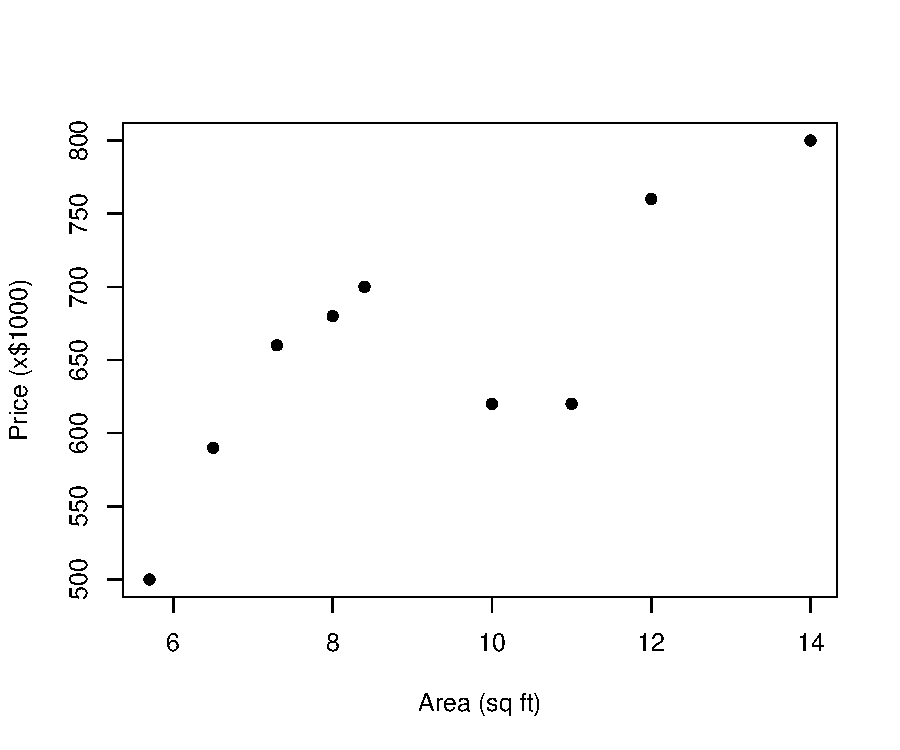
\includegraphics[width=0.6\textwidth]{section16/images/utm_apartments.pdf}
    \caption{Plot of Price vs Area for Apartments near UTM}
\end{figure}
\begin{table}[H]
\centering
\renewcommand{\arraystretch}{1.4}
\begin{tabular}{|c|c|c|c|c|c|}
\hline
\textbf{Price} & \textbf{Area} & $(x - \bar{x})$ & $(y - \bar{y})$ & $(x - \bar{x})(y - \bar{y})$ & $(x - \bar{x})^2$ \\
\hline
620 & 11.0 & 1.8  & -38.9   & -70.02   & 3.24 \\
590 & 6.5  & -2.7 & -68.9   & 186.03   & 7.29 \\
620 & 10.0 & 0.8  & -38.9   & -31.12   & 0.64 \\
700 & 8.4  & -0.8 & 41.1    & -32.88   & 0.64 \\
680 & 8.0  & -1.2 & 21.1    & -25.32   & 1.44 \\
500 & 5.7  & -3.5 & -158.9  & 556.15   & 12.25 \\
760 & 12.0 & 2.8  & 101.1   & 283.08   & 7.84 \\
800 & 14.0 & 4.8  & 141.1   & 677.28   & 23.04 \\
660 & 7.3  & -1.9 & 1.1     & -2.09    & 3.61 \\
\hline
\textbf{Sum} & 82.9 &       &           & $\sum (x - \bar{x})(y - \bar{y}) = 1541.11$ & $\sum (x - \bar{x})^2 = 60.00$ \\
\hline
\end{tabular}
\caption{Deviation table for computing $\hat{\beta}_1$ and $\hat{\beta}_0$}
\end{table}


\noindent The sample means are:
\[
\bar{y} = \frac{\sum y}{n} = \frac{5930}{9} = 658.89, \qquad
\bar{x} = \frac{\sum x}{n} = \frac{82.9}{9} = 9.21
\]
\subsubsection*{Finding the Regression Coefficients}

To compute the least squares regression line, we calculate the slope and intercept using the formulas:

\[
\hat{\beta}_1 = \frac{S_{xy}}{S_{xx}} = \frac{1541.11}{60} = 25.69
\]
\[
\hat{\beta}_0 = \bar{y} - \hat{\beta}_1 \bar{x} = 658.89 - (25.69)(9.21) = 422.28
\]

\subsubsection*{Equation of the Regression Line}

Using the values above, we write the estimated regression equation as:

\[
\hat{y} = \hat{\beta}_0 + \hat{\beta}_1 x = 422.28 + 25.69x
\]

This equation gives the predicted apartment price (in \$1000s) based on area (in 100 sq ft).

\subsubsection*{Interpretation of Coefficients}

The slope $\hat{\beta}_1 = 25.69$ means that for every additional 100 sq ft in area, we expect the apartment price to increase by approximately \$25,690 on average.\\
The intercept $\hat{\beta}_0 = 422.28$ suggests the predicted price when the area is zero. While this has no practical interpretation in this context, it is a necessary component of the regression model.

\subsubsection*{Interpolation and Extrapolation}

To estimate the price of an apartment with an area of 800 sq ft (i.e., $x = 8$), we compute:

\[
\hat{y} = 422.28 + 25.69(8) = 627.8 \quad (\$1000)
\]

Since 8 is within the range of observed values, this is an example of \textbf{interpolation.}

For an apartment with 2,500 sq ft ($x = 25$):

\[
\hat{y} = 422.28 + 25.69(25) = 1064.53 \quad (\$1000)
\]

This is an example of \textbf{extrapolation}, and such predictions should be treated with caution since they lie outside the data range.\\
We can create a simple linear regression model in R using the \texttt{lm} command:

\noindent\textbf{R code}
\begin{tcolorbox}[colback=gray!10, colframe=black!45, arc=2mm,
  before skip=4pt, after skip=4pt]
\begin{verbatim}
lm(y ~ x, data = data_source)
\end{verbatim}
\end{tcolorbox}

\noindent The data is available in the \texttt{apt\_around\_utm.csv} file.

\noindent\textbf{R code}
\begin{tcolorbox}[colback=gray!10, colframe=black!45, arc=2mm,
  before skip=4pt, after skip=4pt]
\begin{verbatim}
apt = read.csv(file.choose())
# apt = read.csv("~/PATH_TO_FILE/apt_around_utm.csv")

apt_model = lm(price ~ area, data = apt)
\end{verbatim}
\end{tcolorbox}

\noindent\textbf{R output}
\begin{tcolorbox}[colback=gray!10, colframe=black!45, arc=2mm,
  before skip=4pt, after skip=4pt]
\begin{verbatim}
> apt_model

Call:
lm(formula = price ~ area, data = apt)

Coefficients:
(Intercept)       area  
     422.26       25.69  
\end{verbatim}
\end{tcolorbox}

We can compute the residuals and the sum of squared errors (SSE) using the table below:

\begin{center}
\renewcommand{\arraystretch}{1.0}
\begin{tabular}{cccccc}
\toprule
$y$ & $x$ & $\hat{y}$ & $y - \hat{y}$ & $(y - \hat{y})^2$ \\
\midrule
620 & 11.0 & 704.85 & -84.85 & 7198.73 \\
590 & 6.5 & 589.24 & 0.76 & 0.58 \\
620 & 10.0 & 679.16 & -59.16 & 3499.36 \\
700 & 8.4 & 638.05 & 61.95 & 3837.62 \\
680 & 8.0 & 627.78 & 52.22 & 2727.4 \\
500 & 5.7 & 568.69 & -68.69 & 4718.13 \\
760 & 12.0 & 730.54 & 29.46 & 868.17 \\
800 & 14.0 & 781.92 & 18.08 & 327.06 \\
660 & 7.3 & 609.79 & 50.21 & 2520.79 \\
\bottomrule
\end{tabular}
\end{center}

Recall our fitted regression model:
\[
\hat{y} = 25.69x + 422.26
\]

\[
\text{SSE} = \sum (y_i - \hat{y}_i)^2 = 25,\!697.83
\]

We now conduct a hypothesis test on the slope $\beta_1$ at the 5\% significance level.

\textbf{Step 1: Hypotheses}
\[
H_0: \beta_1 = 0 \quad \text{vs.} \quad H_a: \beta_1 \ne 0
\]

\textbf{Step 2: Test statistic}
\[
s^2 = \frac{SSE}{n - 2} = \frac{25,\!697.83}{7} = 3670.26
\]
\[
s = \sqrt{3670.26} = 60.58
\]
\[
SE(\hat{\beta}_1) = \frac{s}{\sqrt{S_{xx}}} = \frac{60.58}{\sqrt{60}} = 7.82
\]
\[
t = \frac{\hat{\beta}_1 - 0}{SE(\hat{\beta}_1)} = \frac{25.69}{7.82} = 3.284
\]

\textbf{Step 3: Conclusion}
Using $t$-distribution with 7 degrees of freedom:

\[
0.005 < p\text{-value} < 0.01
\]

Since $p$-value $< 0.05$, we reject $H_0$ and conclude that there is sufficient evidence that $\beta_1 \ne 0$.This suggests there is a statistically significant relationship between price and area for apartments near UTM.

\textbf{Final Check: Total Sum of Squares}

\begin{center}
\renewcommand{\arraystretch}{1.2}
\begin{tabular}{ccccccc}
\toprule
$y$ & $x$ & $\hat{y}$ & $(y - \hat{y})^2$ & $(y - \bar{y})^2$ & $(\hat{y} - \bar{y})^2$ \\
\midrule
620 & 11.0 & 704.85 & 7198.73 & 2112.00 & 1512.35 \\
590 & 6.5 & 589.24 & 0.58 & 4850.88 & 4745.68 \\
620 & 10.0 & 679.16 & 3499.36 & 410.73 & 1512.35 \\
700 & 8.4 & 638.05 & 3837.62 & 434.20 & 1690.12 \\
680 & 8.0 & 627.78 & 2727.4 & 968.04 & 445.68 \\
500 & 5.7 & 568.69 & 4718.13 & 8136.08 & 2524.68 \\
760 & 12.0 & 730.54 & 868.17 & 5133.21 & 10223.46 \\
800 & 14.0 & 781.92 & 327.06 & 1513.47 & 19912.35 \\
660 & 7.3 & 609.79 & 2520.79 & 2410.45 & 1.23 \\
\bottomrule
\end{tabular}
\end{center}

\[
SSE + SSR = SST = 25,\!697.83 + 39,\!591.06 = 65,\!288.90
\]
This confirms the ANOVA identity: Total = Explained + Residual

We previously estimated the model:

\[
\hat{y} = 25.69x + 422.26
\]

\textbf{Coefficient of Determination and Correlation}

\[
r^2 = \frac{SSR}{SST} = \frac{39591.06}{65288.90} = 0.6063 = 60.63\%
\]

Interpretation: Approximately 60.63\% of the variability in price is explained by the regression model.

\[
r = \pm \sqrt{r^2} = \pm \sqrt{0.6063} = \pm 0.779
\]

Since \( \hat{\beta}_1 > 0 \), we choose the positive root:

\[
r = 0.779
\]

Interpretation: There is a strong positive correlation between apartment area and price.

\noindent\textbf{R code}
\begin{tcolorbox}[colback=gray!10, colframe=black!45, arc=2mm]
\begin{verbatim}
model = lm(y~x, data = data\_source) 
summary(model)
\end{verbatim}
\end{tcolorbox}

\noindent\textbf{R code}
\begin{tcolorbox}[colback=gray!10, colframe=black!45, arc=2mm]
\begin{verbatim}
apt\_model = lm(price ~ area, data = apt)
summary(apt\_model)
\end{verbatim}
\end{tcolorbox}

\noindent\textbf{R code}
\begin{tcolorbox}[colback=gray!10, colframe=black!45, arc=2mm]
\begin{verbatim}
Call:
lm(formula = price ~ area, data = apt)

Coefficients:
            Estimate Std. Error t value Pr(>|t|)
(Intercept)  422.256   74.834     5.643  0.00078 ***
area         25.690    7.823      3.284  0.01341 *

Residual standard error: 60.59 on 7 degrees of freedom
Multiple R-squared: 0.6064,    Adjusted R-squared: 0.5502 
F-statistic: 10.78 on 1 and 7 DF,  p-value: 0.01341
\end{verbatim}
\end{tcolorbox}

\textbf{Two-sided Test for Slope Coefficient}

By default, R performs a two-sided test:
\[
H_0: \beta_1 = 0 \quad \text{vs.} \quad H_a: \beta_1 \neq 0
\]

\vspace{0.3cm}

Test statistic:
\[
t^* = \frac{\hat{\beta}_1 - 0}{SE(\hat{\beta}_1)} = \frac{25.690 - 0}{7.823} = 3.284
\]

\[
t^* \sim t_{(n - 2)}  \quad \text{with } df = 9 - 2 = 7
\]

\vspace{0.5cm}

\textbf{p-value} is the total shaded area in both tails. From R output:
\[
\text{p-value} = 0.01341
\]

\end{example}
\begin{definition}[Interpolation and Extrapolation]
\vspace{-1em}
\begin{itemize}
    \item{\textbf{Interpolation}} is calculating predicted values of $y$ using our linear model while working within the range of $x$ in which data was available to construct our model.
    
    \item{\textbf{Extrapolation}} is calculating predicted values of $y$ using our linear model outside the range of $x$ used to obtain the linear model.
    
    \item Interpolation is usually safe if we have a good linear model.
    
    \item Extrapolation must be performed carefully since extrapolations that are done without any foresight can be very inaccurate.
\end{itemize}
\end{definition}
\section{Residual Plots}

Residual plots are used to verify assumptions related to the error terms in a regression model.

\[
Y = \beta_0 + \beta_1 X + \varepsilon, \quad \varepsilon \sim \mathcal{N}(0, \sigma^2)
\]

The assumption $\varepsilon \sim \mathcal{N}(0, \sigma^2)$ implies:
\begin{itemize}
    \item Mean of errors is 0
    \item Constant variance of errors (homoscedasticity)
\end{itemize}

\vspace{0.5em}
We plot the residuals:
\[
e_i = y_i - \hat{y}_i
\]
against the fitted values $\hat{y}_i$ to assess these assumptions.

\vspace{1em}
\subsection*{What to Look for in a Good Residual Plot}

If the assumption $\varepsilon \sim \mathcal{N}(0, \sigma^2)$ is satisfied, the residual plot should have the following features:

\begin{enumerate}
    \item \textbf{Random scattering:} No obvious pattern in residuals.
    \begin{itemize}
        \item A pattern (e.g., curve) may indicate a non-linear relationship.
        \item Random scattering also suggests independence of errors.
    \end{itemize}
    
    \item \textbf{Constant variance:} Residuals should fall within a horizontal band, roughly half above and half below zero.
    \begin{itemize}
        \item Suggests constant variance (homoscedasticity).
    \end{itemize}
    
    \item \textbf{No influential points or clustering:} The plot should not show isolated influential observations or clustering.
\end{enumerate}

\begin{figure}[H]
  \centering
  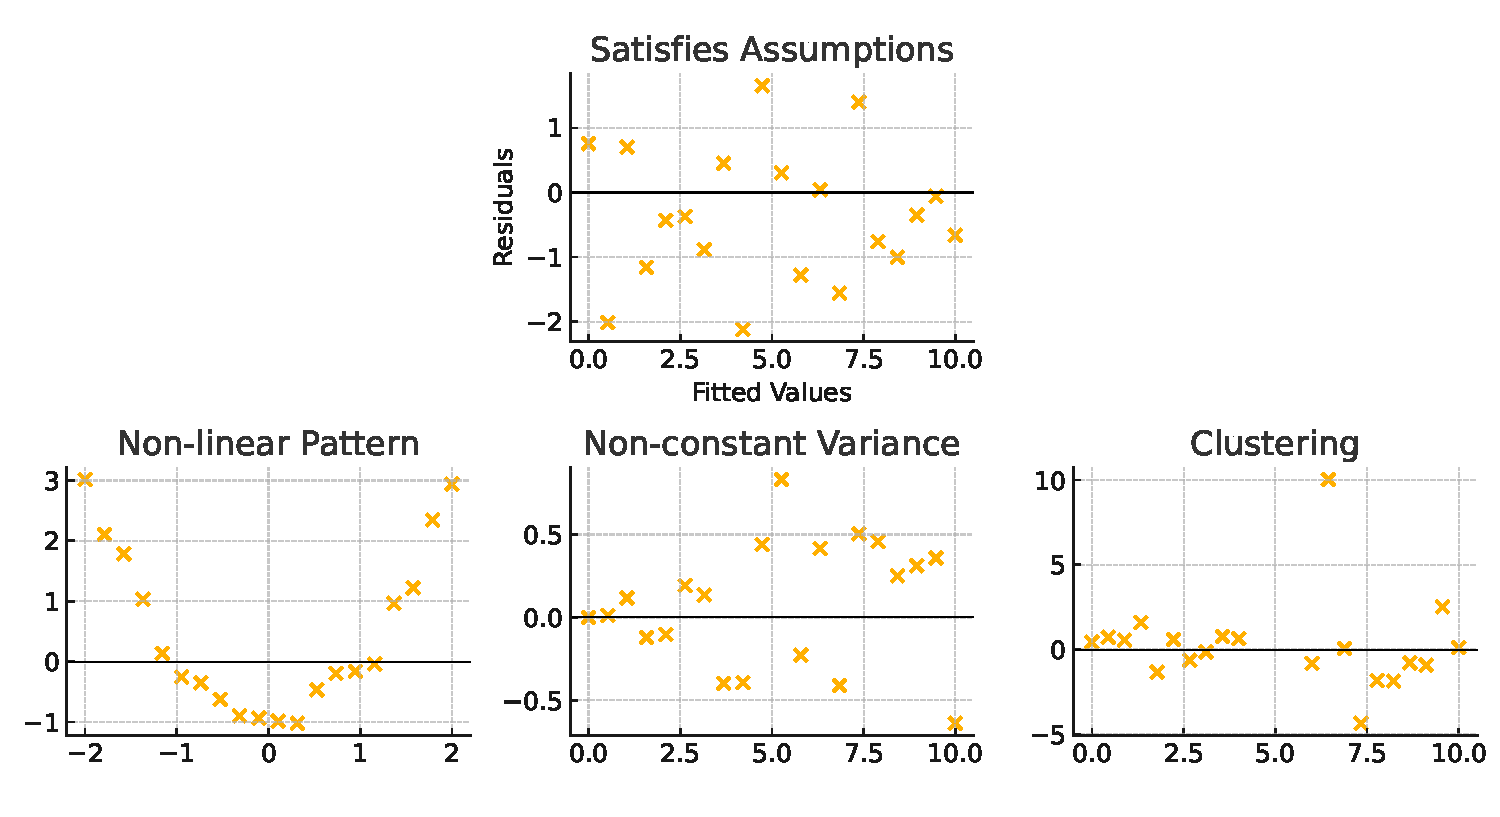
\includegraphics[width=1.0\textwidth]{section16/images/residual_plots.pdf}
  \caption{Residual Plots - Good and Bad Examples}
\end{figure}

\begin{tcolorbox}[colback=yellow!5, colframe=yellow!50!black, title=Assumptions of Simple Linear Regression (SLR)]
    The model is: \quad $Y = \beta_0 + \beta_1 X + \varepsilon$, \quad where $\varepsilon \sim \mathcal{N}(0, \sigma^2)$
 \begin{itemize}
    \item The relationship between $X$ and $Y$ is linear.
    
    \item Residuals:
    \begin{itemize}
        \item are independent
        \item have constant variance
        \item are normally distributed
    \end{itemize}
    These assumptions can be verified using residual plots.
\end{itemize}
\end{tcolorbox}
\begin{center}
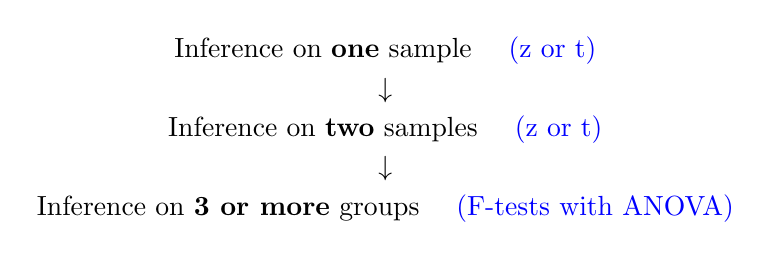
\begin{tikzpicture}[node distance=0.5cm] % much tighter spacing
  \node (one) {Inference on \textbf{one} sample \quad \textcolor{blue}{(z or t)}};
  \node (arrow1) [below of=one] {$\downarrow$};
  \node (two) [below of=arrow1] {Inference on \textbf{two} samples \quad \textcolor{blue}{(z or t)}};
  \node (arrow2) [below of=two] {$\downarrow$};
  \node (three) [below of=arrow2] {Inference on \textbf{3 or more} groups \quad \textcolor{blue}{(F-tests with ANOVA)}};
\end{tikzpicture}
\end{center}